\documentclass[times, twoside]{zHenriquesLab-StyleBioRxiv}
\usepackage{booktabs}
\usepackage{multirow}
\usepackage{siunitx}
\sisetup{detect-all}

% Lead author for running footer
\leadauthor{Weigel}

\begin{document}

\title{Quantitative analysis of extracellular space across tissue preparation methods in volume electron microscopy}
\shorttitle{ECS analysis across EM preparation methods}

% Authors - update as needed
\author[1,\Letter]{Aubrey V. Weigel}
% \author[1]{Second Author}

\affil[1]{HHMI Janelia Research Campus, Ashburn, VA 20147, USA}

\maketitle

\begin{abstract}
The extracellular space (ECS) is a critical compartment for intercellular signaling, molecular transport, and tissue homeostasis, yet its ultrastructural dimensions remain debated due to sensitivity to tissue preparation. Here we present a systematic, multi-metric comparison of ECS morphology between chemical fixation and rapid high-pressure freezing (HPF) across 42 volume electron microscopy crops spanning four mouse tissues (kidney, heart, liver, cortex) from the CellMap open-access dataset. We quantify ECS volume fraction, channel half-width, per-cell surface-area-to-volume ratio, sphericity, inter-cell gap distance via Voronoi tessellation, and local surface curvature from both voxel-based and mesh-based methods. We document each metric's known biases and artifacts, including a pervasive confound between voxel resolution (2--8\,nm) and preparation type that limits the interpretability of direct comparisons. This work provides a reproducible analytical framework and baseline measurements for future studies of ECS ultrastructure.
\end{abstract}

\begin{keywords}
extracellular space | electron microscopy | high-pressure freezing | chemical fixation | tissue ultrastructure | image analysis
\end{keywords}

\begin{corrauthor}
weigela\at janelia.hhmi.org
\end{corrauthor}

%% ============================================================
\section*{Introduction}
%% ============================================================

The extracellular space (ECS) occupies a significant fraction of tissue volume and plays essential roles in molecular diffusion, cell-cell communication, and ion homeostasis \cite{Sykova2008, Nicholson2001}. In the brain, the ECS is estimated to comprise approximately 20\% of tissue volume in vivo, yet early electron microscopy (EM) studies using conventional chemical fixation reported much smaller values (3--5\%), leading to a longstanding debate about the extent to which tissue preparation artifacts distort ECS measurements \cite{VanHarreveld1972}.

Rapid high-pressure freezing (HPF) followed by freeze substitution has been proposed as a more faithful preservation method, avoiding the osmotic perturbations and dehydration artifacts inherent in aldehyde-based chemical fixation \cite{Studer2008}. Several studies have directly compared the two methods and reported larger ECS in HPF-prepared tissue, particularly in brain \cite{Korogod2015}. However, these comparisons have generally been limited to a single tissue type and a small number of metrics.

The CellMap project \cite{Heinrich2021, Xu2021} provides an open-access collection of volume EM datasets with dense ground-truth segmentation of cellular organelles and extracellular space across multiple mouse tissues, prepared by both chemical fixation and rapid HPF. This resource enables a systematic, multi-metric comparison of ECS morphology across preparation methods and tissue types.

Here we analyze 42 annotated crops from four tissues (kidney, heart, liver, cortex) using nine complementary metrics that characterize ECS volume, geometry, cell morphology, intercellular contacts, and membrane curvature. For each metric, we report the methods, results, known biases, and artifacts. We emphasize a critical confound in this dataset: voxel resolution is perfectly correlated with preparation type (chemical = 2--4\,nm, HPF = 8\,nm), making it impossible to cleanly attribute observed differences to biology versus resolution.

%% ============================================================
\section*{Methods}
%% ============================================================

\subsection*{Data source}
All data were obtained from the CellMap open-access volume EM collection \cite{Heinrich2021, Xu2021}. We analyzed 42 ground-truth annotated crops from 8 datasets spanning 4 mouse tissues and 2 preparation methods (Table~\ref{tab:datasets}). Segmentation labels included semantic ECS masks (binary: 0/1) and instance cell segmentation masks (0 = absent, nonzero = cell ID). Voxel sizes ranged from 2\,nm to 8\,nm isotropic.

\subsection*{ECS volume fraction}
For each crop, the number of voxels labeled as ECS and as cell were counted directly from the segmentation arrays. ECS volume fraction was computed as ECS voxels / total crop voxels $\times$ 100\%.

\subsection*{ECS channel half-width}
A Euclidean distance transform was applied to the binary ECS mask, with cell voxels as the reference surface. Each ECS voxel received a value equal to its distance (in nm) to the nearest cell boundary. To exclude vessel lumens and other large open spaces, values were filtered to $<$200\,nm. Summary statistics (median, mean, percentiles, standard deviation) and cumulative fractions below thresholds (10, 20, 30, 50, 75, 100\,nm) were computed per crop.

\subsection*{Per-cell morphology}
For each segmented cell, volume was computed as voxel count $\times$ voxel volume. Surface area was computed by face-counting on the cubic voxel grid: each voxel face abutting ECS was counted as one unit of ECS-facing surface area. The surface-area-to-volume ratio (SA:V) was computed in units of 1/nm. Sphericity was computed as $\psi = \pi^{1/3} (6V)^{2/3} / A$, where $V$ is volume and $A$ is total surface area (all faces, not just ECS-facing).

To control for voxel-size effects on face-counting, a resolution-normalized version was computed by resampling all segmentation masks to 8\,nm isotropic voxels before analysis.

\subsection*{Inter-cell gap distance (Voronoi)}
ECS voxels were assigned to their nearest cell via the distance transform, creating a Voronoi tessellation of the extracellular space. At boundaries where two cells' Voronoi territories met, the gap width was computed as the sum of both cells' distance contributions. Per-crop summary statistics and contact fractions at thresholds (10, 20, 40, 80, 160, 320\,nm) were reported.

\subsection*{Surface curvature --- voxel-based}
The binary cell mask was smoothed with a Gaussian kernel ($\sigma$ = 16\,nm physical) and mean curvature $H$ was computed at each surface voxel using the level-set formula on the gradient and Hessian of the smoothed field. Positive $H$ = convex (bulging into ECS), negative $H$ = concave (invagination). Only ECS-facing surface voxels were analyzed. Per-cell statistics included median $|H|$, fraction convex, and median radius of curvature ($1/|H|$). Cells below 2.56$\times 10^6$\,nm$^3$ volume were excluded.

\subsection*{Surface curvature --- mesh-based}
A triangulated isosurface was extracted from each cell's binary mask using the marching cubes algorithm, with 1-voxel Gaussian pre-smoothing. Mean curvature $H$ was computed at each mesh vertex from the discrete Laplace--Beltrami operator. Only ECS-facing vertices were retained, defined as vertices whose nearest non-self segmentation label was ECS rather than another cell. Per-cell statistics were computed as for the voxel-based method. Mesh quality metadata (vertex count, face count, ECS vertex count) were recorded.

\subsection*{Statistical analysis}
Group comparisons between Chemical and HPF preparations used the Mann--Whitney $U$ test (two-sided). Correlations between metrics and voxel size were assessed using Spearman's rank correlation. No multiple-comparison corrections were applied; $p$-values are reported as descriptive statistics.

%% ============================================================
\section*{Results}
%% ============================================================

\subsection*{Global confound: voxel size and preparation type are perfectly correlated}
All Chemical fixation crops were imaged at 2\,nm (7 crops) or 4\,nm (14 crops) isotropic voxels, with 3 crops at 8\,nm. All HPF crops were imaged at 8\,nm (17 crops). There is effectively no overlap in resolution between the two preparation types (Table~\ref{tab:datasets}). Per-cell metrics showed significant correlations with voxel size: SA:V ($r = -0.30$, $p < 10^{-25}$), sphericity ($r = -0.17$, $p < 10^{-8}$), and curvature ($r = +0.13$, $p < 10^{-4}$; Spearman). Any comparison between Chemical and HPF is simultaneously a comparison between high and low resolution.

\subsection*{ECS volume fraction}
Across all tissues, Chemical crops had a higher median ECS fraction (20.1\%, IQR 13.1--31.8\%, $n = 24$) than HPF (9.6\%, IQR 3.9--14.7\%, $n = 17$; Mann--Whitney $p = 0.019$). Within-group variance was large: Chemical ranged from 1.4\% to 74.6\%. By tissue, liver showed the largest separation (Chemical 27.1 $\pm$ 4.5\% vs HPF 7.5 $\pm$ 2.5\%), while cortex showed the reverse (Chemical 13.3 $\pm$ 3.5\% vs HPF 32.9 $\pm$ 15.0\%; Table~\ref{tab:ecs_volume}).

\subsection*{ECS channel half-width}
The overall mean narrow-ECS median half-width was 25.4\,nm for Chemical ($n = 24$) and 21.6\,nm for HPF ($n = 17$). However, within Chemical crops alone, 2\,nm-voxel crops reported a mean narrow median of 13.9\,nm with 82.0\% of ECS below 20\,nm, while 4\,nm-voxel crops reported 29.7\,nm with 44.8\% below 20\,nm, and 8\,nm-voxel crops reported 32.5\,nm with 33.8\% below 20\,nm (Table~\ref{tab:ecs_width}). This monotonic dependence on voxel size within a single preparation type demonstrates that resolution dominates the signal at fine thresholds.

\subsection*{Per-cell morphology}
Using resolution-normalized data (8\,nm isotropic), Chemical cells had higher SA:V than HPF at no filter (0.050 vs 0.043), but the direction depended on the minimum cell-size threshold: at $\geq$0.05\,$\mu$m$^3$, Chemical SA:V was lower (0.015 vs 0.019, $p = 0.002$). Sphericity was consistently higher in Chemical cells across all size filters (0.57 vs 0.48 at $\geq$0.01\,$\mu$m$^3$, $p < 0.0001$). Of 1,179 native-resolution cells, 601 (51\%) were below 0.01\,$\mu$m$^3$ and 158 had 100\% ECS-facing surface, indicating boundary-truncated fragments.

By tissue at native resolution (volume filter $>$2.56$\times 10^6$\,nm$^3$): liver and cortex showed no SA:V difference between preparations (both 0.039 and 0.032--0.033, respectively), while kidney showed Chemical $>$ HPF (0.038 vs 0.027; Table~\ref{tab:morphology}).

\subsection*{Inter-cell gap distance}
Chemical crops had a mean Voronoi gap median of 48.5\,nm ($n = 24$) and HPF 52.5\,nm ($n = 17$). The contact fraction at 20\,nm was 0.308 for Chemical and 0.000 for HPF. However, all three Chemical crops at 8\,nm voxels also showed contact\_frac\_20nm $= 0.000$, identical to HPF. At 80\,nm, contact fractions were similar (Chemical 0.720, HPF 0.773), consistent with comparable cell packing at scales above the resolution floor.

\subsection*{Surface curvature}
Voxel-based curvature showed Chemical cells with higher median $|H|$ (0.00654 vs 0.00523\,/nm) and smaller radius of curvature (153 vs 191\,nm), with 87\% vs 85\% concave surface.

Mesh-based curvature showed much closer agreement between preparations when unfiltered: median $|H|$ was 0.01066 (Chemical) vs 0.01046\,/nm (HPF), with 82\% vs 83\% concave. After size filtering ($\geq$0.01\,$\mu$m$^3$), a difference emerged: Chemical $|H| = 0.00659$ (radius 152\,nm) vs HPF $|H| = 0.00862$ (radius 116\,nm, $p < 0.0001$). Chemical cells showed more convex surface at all size filters (18--42\% vs 17--32\%).

The two curvature methods disagreed in magnitude: mesh-based $|H|$ was approximately 2$\times$ the voxel-based value, and mesh radius was approximately 60\% smaller (Table~\ref{tab:curvature}).

%% ============================================================
\section*{Discussion}
%% ============================================================

% TODO: Discussion to be written

%% ============================================================
\section*{Known Biases and Artifacts}
%% ============================================================

\subsection*{Voxel resolution confound}
The most significant limitation of this analysis is the perfect confounding of voxel size with preparation type. Chemical crops are 2--4$\times$ higher resolution than HPF crops. This affects every metric: surface area is overestimated at finer voxels (staircase effect), distance transforms have different quantization floors, and curvature computation depends on the effective smoothing scale relative to voxel size. Normalization to 8\,nm isotropic controls for voxel-size effects on face-counting but introduces smoothing artifacts that change absolute values (sphericity increases from 0.52 to 0.65 after normalization).

\subsection*{Crop placement}
Crops were not placed at matched anatomical locations between preparations. A crop on a vessel lumen versus dense parenchyma can differ in ECS fraction by 10--50$\times$. The within-Chemical ECS range of 1.4--74.6\% demonstrates that crop placement variance far exceeds any plausible preparation effect.

\subsection*{Boundary-truncated cells}
Cells intersecting crop boundaries are sliced, creating artificial flat faces that inflate SA:V and reduce sphericity. The 601 cells below 0.01\,$\mu$m$^3$ and 158 cells with 100\% ECS-facing surface are likely fragments. Results depend on the minimum size filter applied, and SA:V direction reverses between Chemical and HPF depending on threshold.

\subsection*{Distance quantization}
At 8\,nm voxels, the minimum resolvable distance is approximately one voxel (8\,nm) for the distance transform and approximately 14\,nm for Voronoi gap measurements ($2 \times$ half-diagonal). This creates a hard floor below which no measurements exist. The observation that Chemical 8\,nm crops show identical contact\_frac\_20nm (0.000) to HPF 8\,nm crops confirms that the Chemical-vs-HPF difference at 20\,nm is a resolution artifact.

\subsection*{Curvature method disagreement}
Voxel-based and mesh-based curvature differ by approximately 2$\times$ in magnitude. Voxel-based curvature suffers from staircase noise on the binary grid; mesh-based curvature introduces implicit smoothing from marching cubes. Both methods show strong concavity bias (82--87\% concave), which may partly reflect real cell-cell wrapping geometry but is also influenced by the preferential sampling of ECS-facing vertices at membrane invaginations.

\subsection*{Discarded metric}
Boundary-based contact fraction (the fraction of crops where any two cell boundary voxels come within $X$\,nm) returned 1.000 at all thresholds $\geq$20\,nm for all crops and was discarded as uninformative.

%% ============================================================
%% TABLES
%% ============================================================

\begin{table*}[t]
\centering
\caption{Datasets analyzed. All voxel sizes are isotropic.}
\label{tab:datasets}
\begin{tabular}{llllr}
\toprule
Dataset & Tissue & Prep & Voxel (nm) & Crops \\
\midrule
jrc\_mus-kidney     & Kidney & Chemical  & 4 & 7 \\
jrc\_mus-kidney-4   & Kidney & Rapid HPF & 8 & 4 \\
jrc\_mus-heart-6    & Heart  & Chemical  & 8 & 3 \\
jrc\_mus-liver      & Liver  & Chemical  & 4 & 7 \\
jrc\_mus-liver-8    & Liver  & Rapid HPF & 8 & 10 \\
jrc\_mus-cortex-2   & Cortex & Rapid HPF & 8 & 2 \\
jrc\_mus-cortex-3   & Cortex & Chemical  & 2 & 7 \\
jrc\_mus-cortex-4   & Cortex & Rapid HPF & 8 & 2 \\
\bottomrule
\end{tabular}
\end{table*}

\begin{table*}[t]
\centering
\caption{ECS volume fraction by tissue and preparation. Values are mean $\pm$ SEM.}
\label{tab:ecs_volume}
\begin{tabular}{lll}
\toprule
Tissue & Chemical & Rapid HPF \\
\midrule
Kidney & 34.4 $\pm$ 9.0\% ($n=7$)  & 24.8 $\pm$ 11.6\% ($n=4$) \\
Heart  & 21.0 $\pm$ 4.8\% ($n=3$)  & N/A \\
Liver  & 27.1 $\pm$ 4.5\% ($n=7$)  & 7.5 $\pm$ 2.5\% ($n=10$) \\
Cortex & 13.3 $\pm$ 3.5\% ($n=7$)  & 32.9 $\pm$ 15.0\% ($n=3$) \\
\bottomrule
\end{tabular}
\end{table*}

\begin{table*}[t]
\centering
\caption{ECS narrow half-width by voxel size, demonstrating resolution dependence within Chemical fixation. Narrow = filtered to $<$200\,nm.}
\label{tab:ecs_width}
\begin{tabular}{llrrr}
\toprule
Voxel (nm) & Prep & $n$ & Mean narrow median (nm) & Mean frac $<$20\,nm \\
\midrule
2 & Chemical  &  7 & 13.9 & 0.820 \\
4 & Chemical  & 14 & 29.7 & 0.448 \\
8 & Chemical  &  3 & 32.5 & 0.338 \\
8 & Rapid HPF & 17 & 21.6 & 0.621 \\
\bottomrule
\end{tabular}
\end{table*}

\begin{table*}[t]
\centering
\caption{Per-cell SA:V ratio by tissue at native resolution (volume filter $>$2.56$\times 10^6$\,nm$^3$). Values are mean $\pm$ SEM in units of 1/nm.}
\label{tab:morphology}
\begin{tabular}{lll}
\toprule
Tissue & Chemical & Rapid HPF \\
\midrule
Kidney & 0.038 $\pm$ 0.001 ($n=230$) & 0.027 $\pm$ 0.002 ($n=81$) \\
Heart  & 0.010 $\pm$ 0.002 ($n=11$)  & N/A \\
Liver  & 0.039 $\pm$ 0.002 ($n=83$)  & 0.039 $\pm$ 0.002 ($n=142$) \\
Cortex & 0.032 $\pm$ 0.002 ($n=101$) & 0.033 $\pm$ 0.001 ($n=326$) \\
\bottomrule
\end{tabular}
\end{table*}

\begin{table*}[t]
\centering
\caption{Surface curvature comparison: voxel-based vs mesh-based methods. Values are medians across cells (all tissues pooled, cells $>$2.56$\times 10^6$\,nm$^3$).}
\label{tab:curvature}
\begin{tabular}{lrrrr}
\toprule
 & \multicolumn{2}{c}{Voxel-based} & \multicolumn{2}{c}{Mesh-based} \\
\cmidrule(lr){2-3} \cmidrule(lr){4-5}
Metric & Chemical & HPF & Chemical & HPF \\
\midrule
Median $|H|$ (1/nm) & 0.00654 & 0.00523 & 0.01066 & 0.01046 \\
Median radius (nm) & 153 & 191 & 94 & 96 \\
Fraction convex (\%) & 12.7 & 14.7 & 18.1 & 17.1 \\
Fraction concave (\%) & 87.3 & 85.3 & 81.9 & 82.9 \\
\bottomrule
\end{tabular}
\end{table*}

%% ============================================================
%% FIGURES
%% ============================================================

\begin{figure*}[t]
\centering
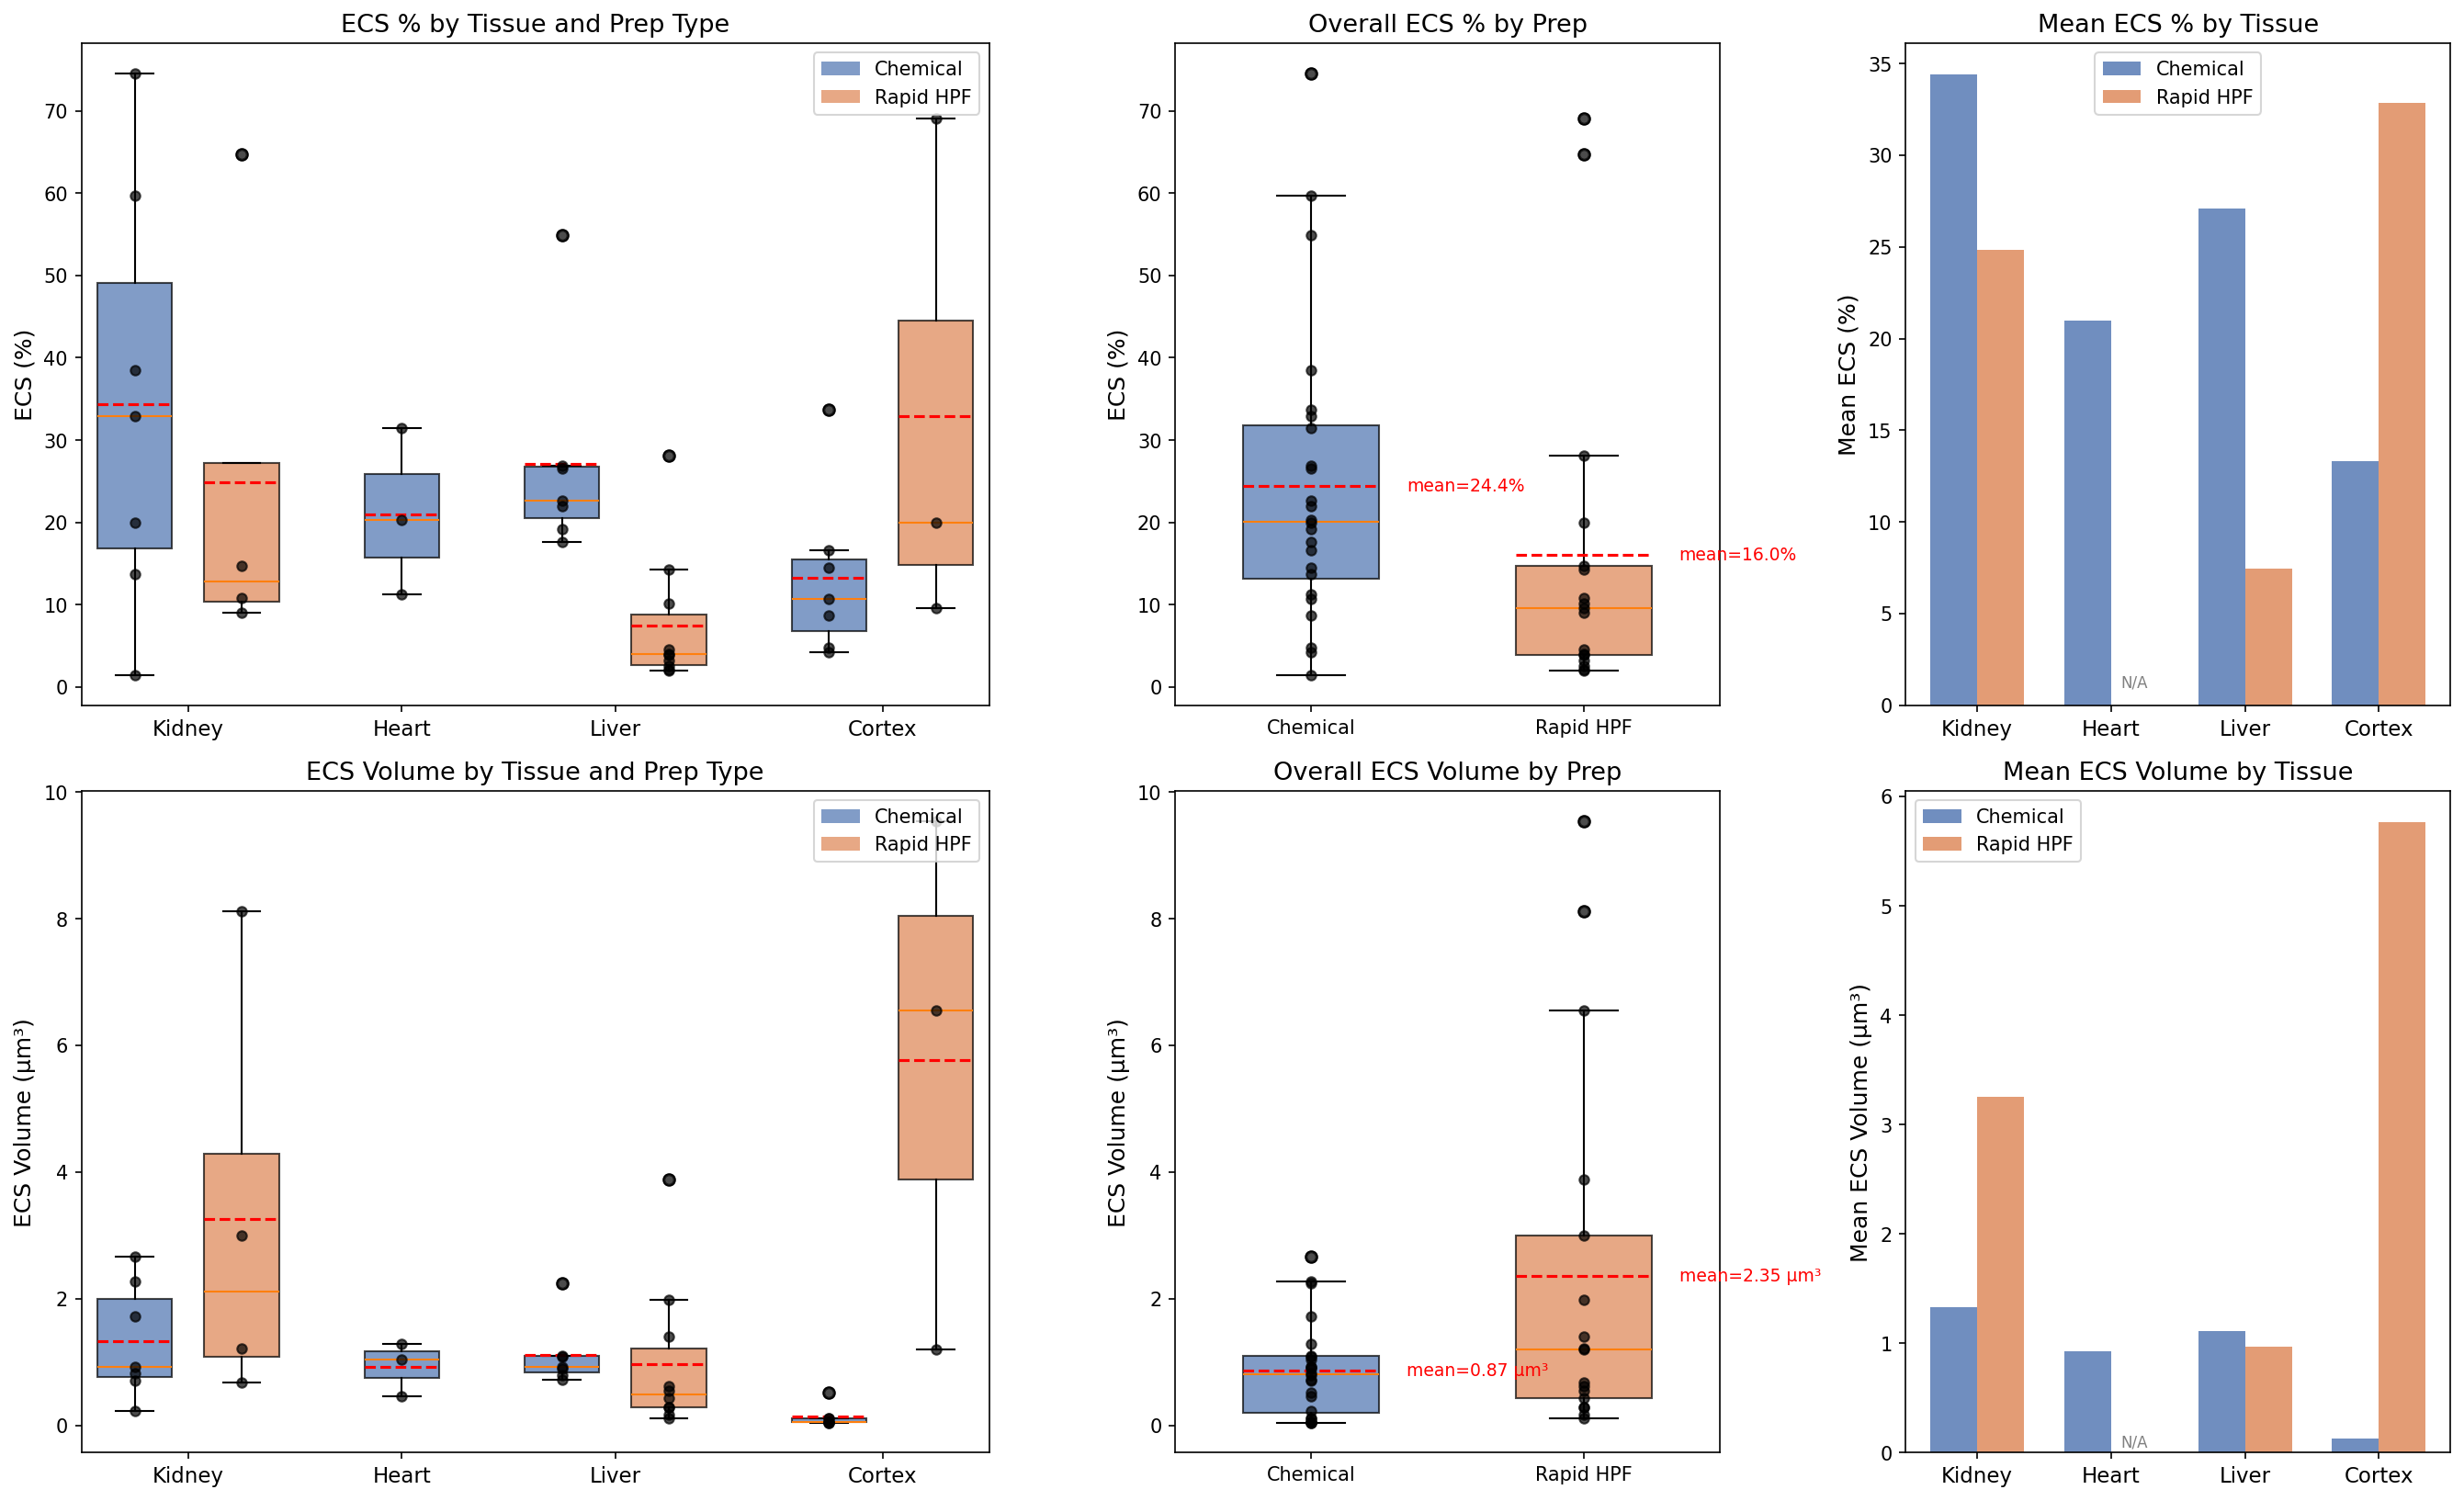
\includegraphics[width=0.95\linewidth]{Figures/ecs_by_prep_type.png}
\caption{ECS volume fraction by tissue and preparation type. Each point represents one crop.}
\label{fig:ecs_volume}
\end{figure*}

\begin{figure*}[t]
\centering
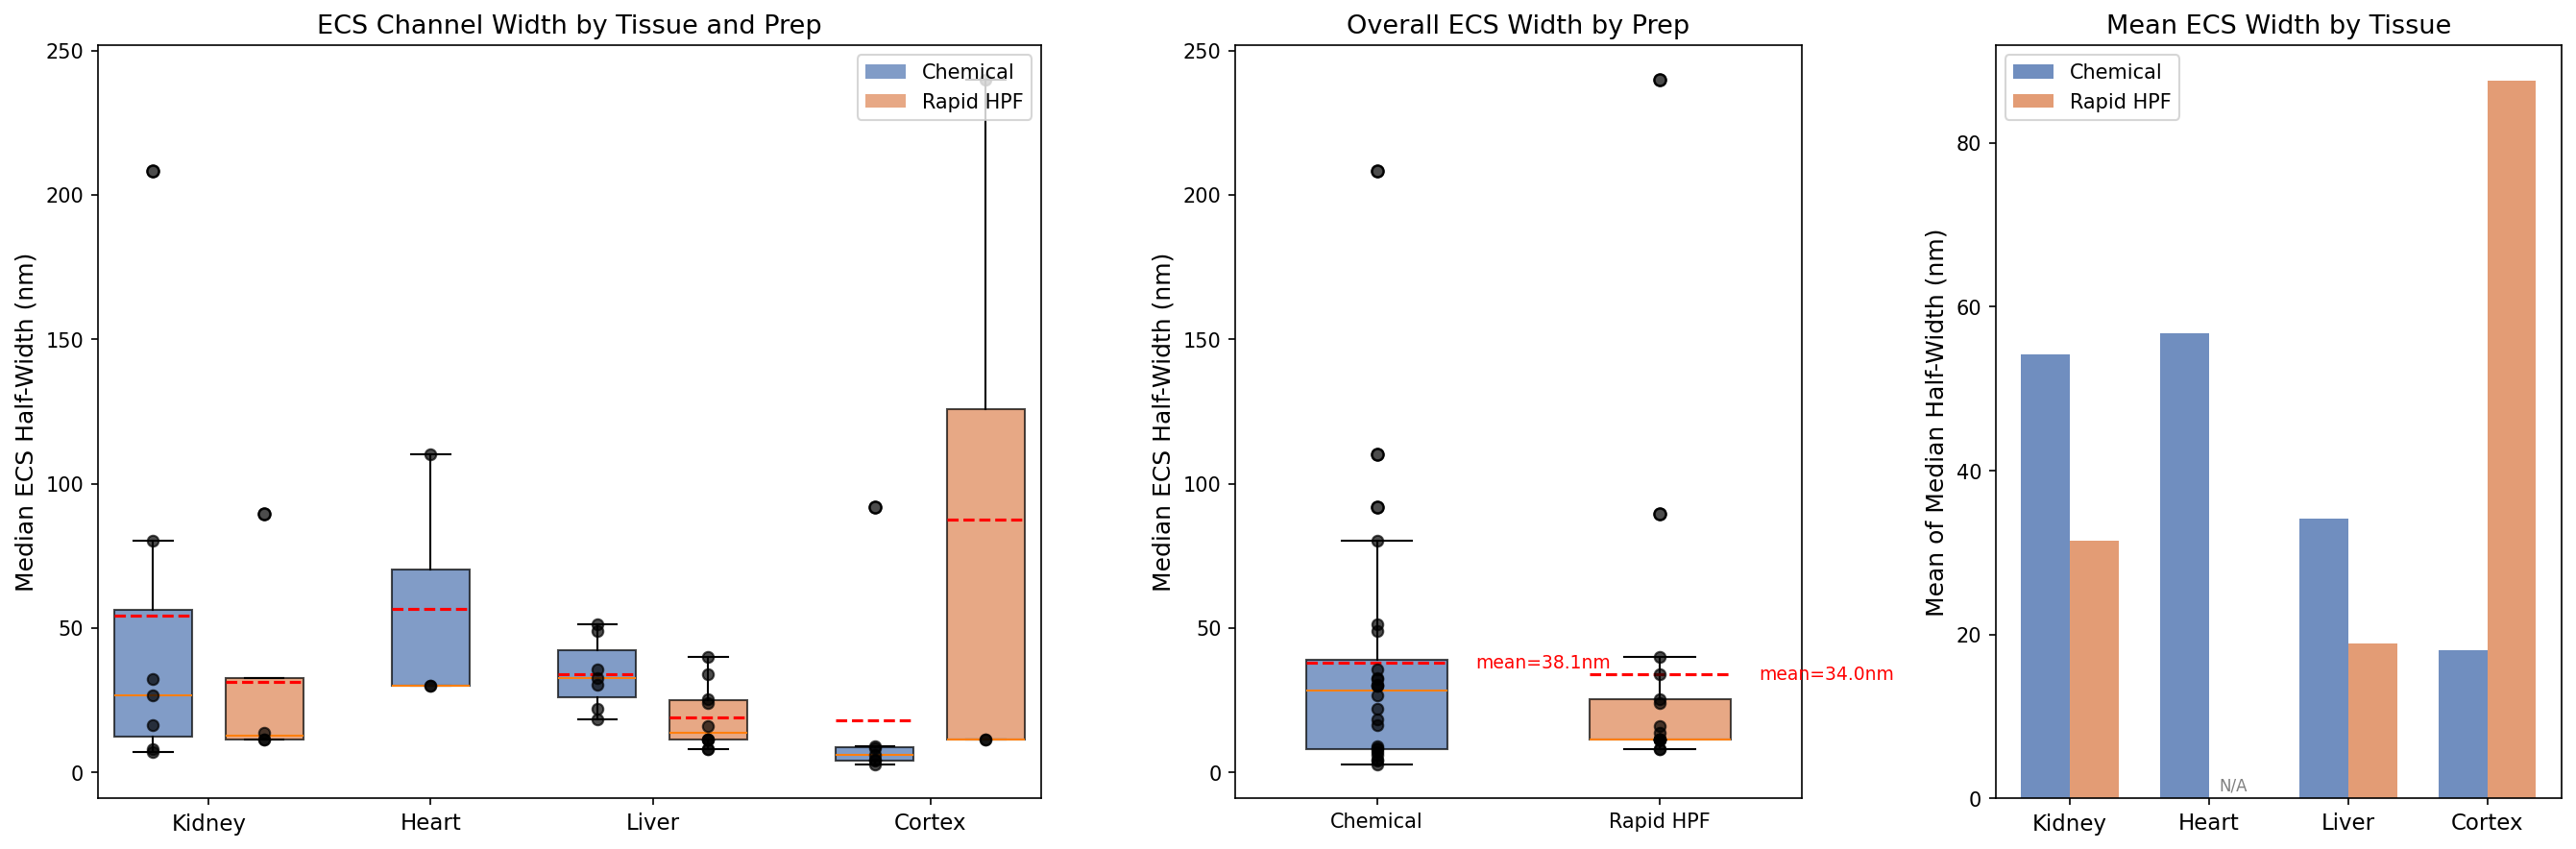
\includegraphics[width=0.95\linewidth]{Figures/ecs_width_by_prep.png}
\caption{ECS channel half-width distributions by preparation type. Filtered to narrow ECS ($<$200\,nm half-width).}
\label{fig:ecs_width}
\end{figure*}

\begin{figure*}[t]
\centering
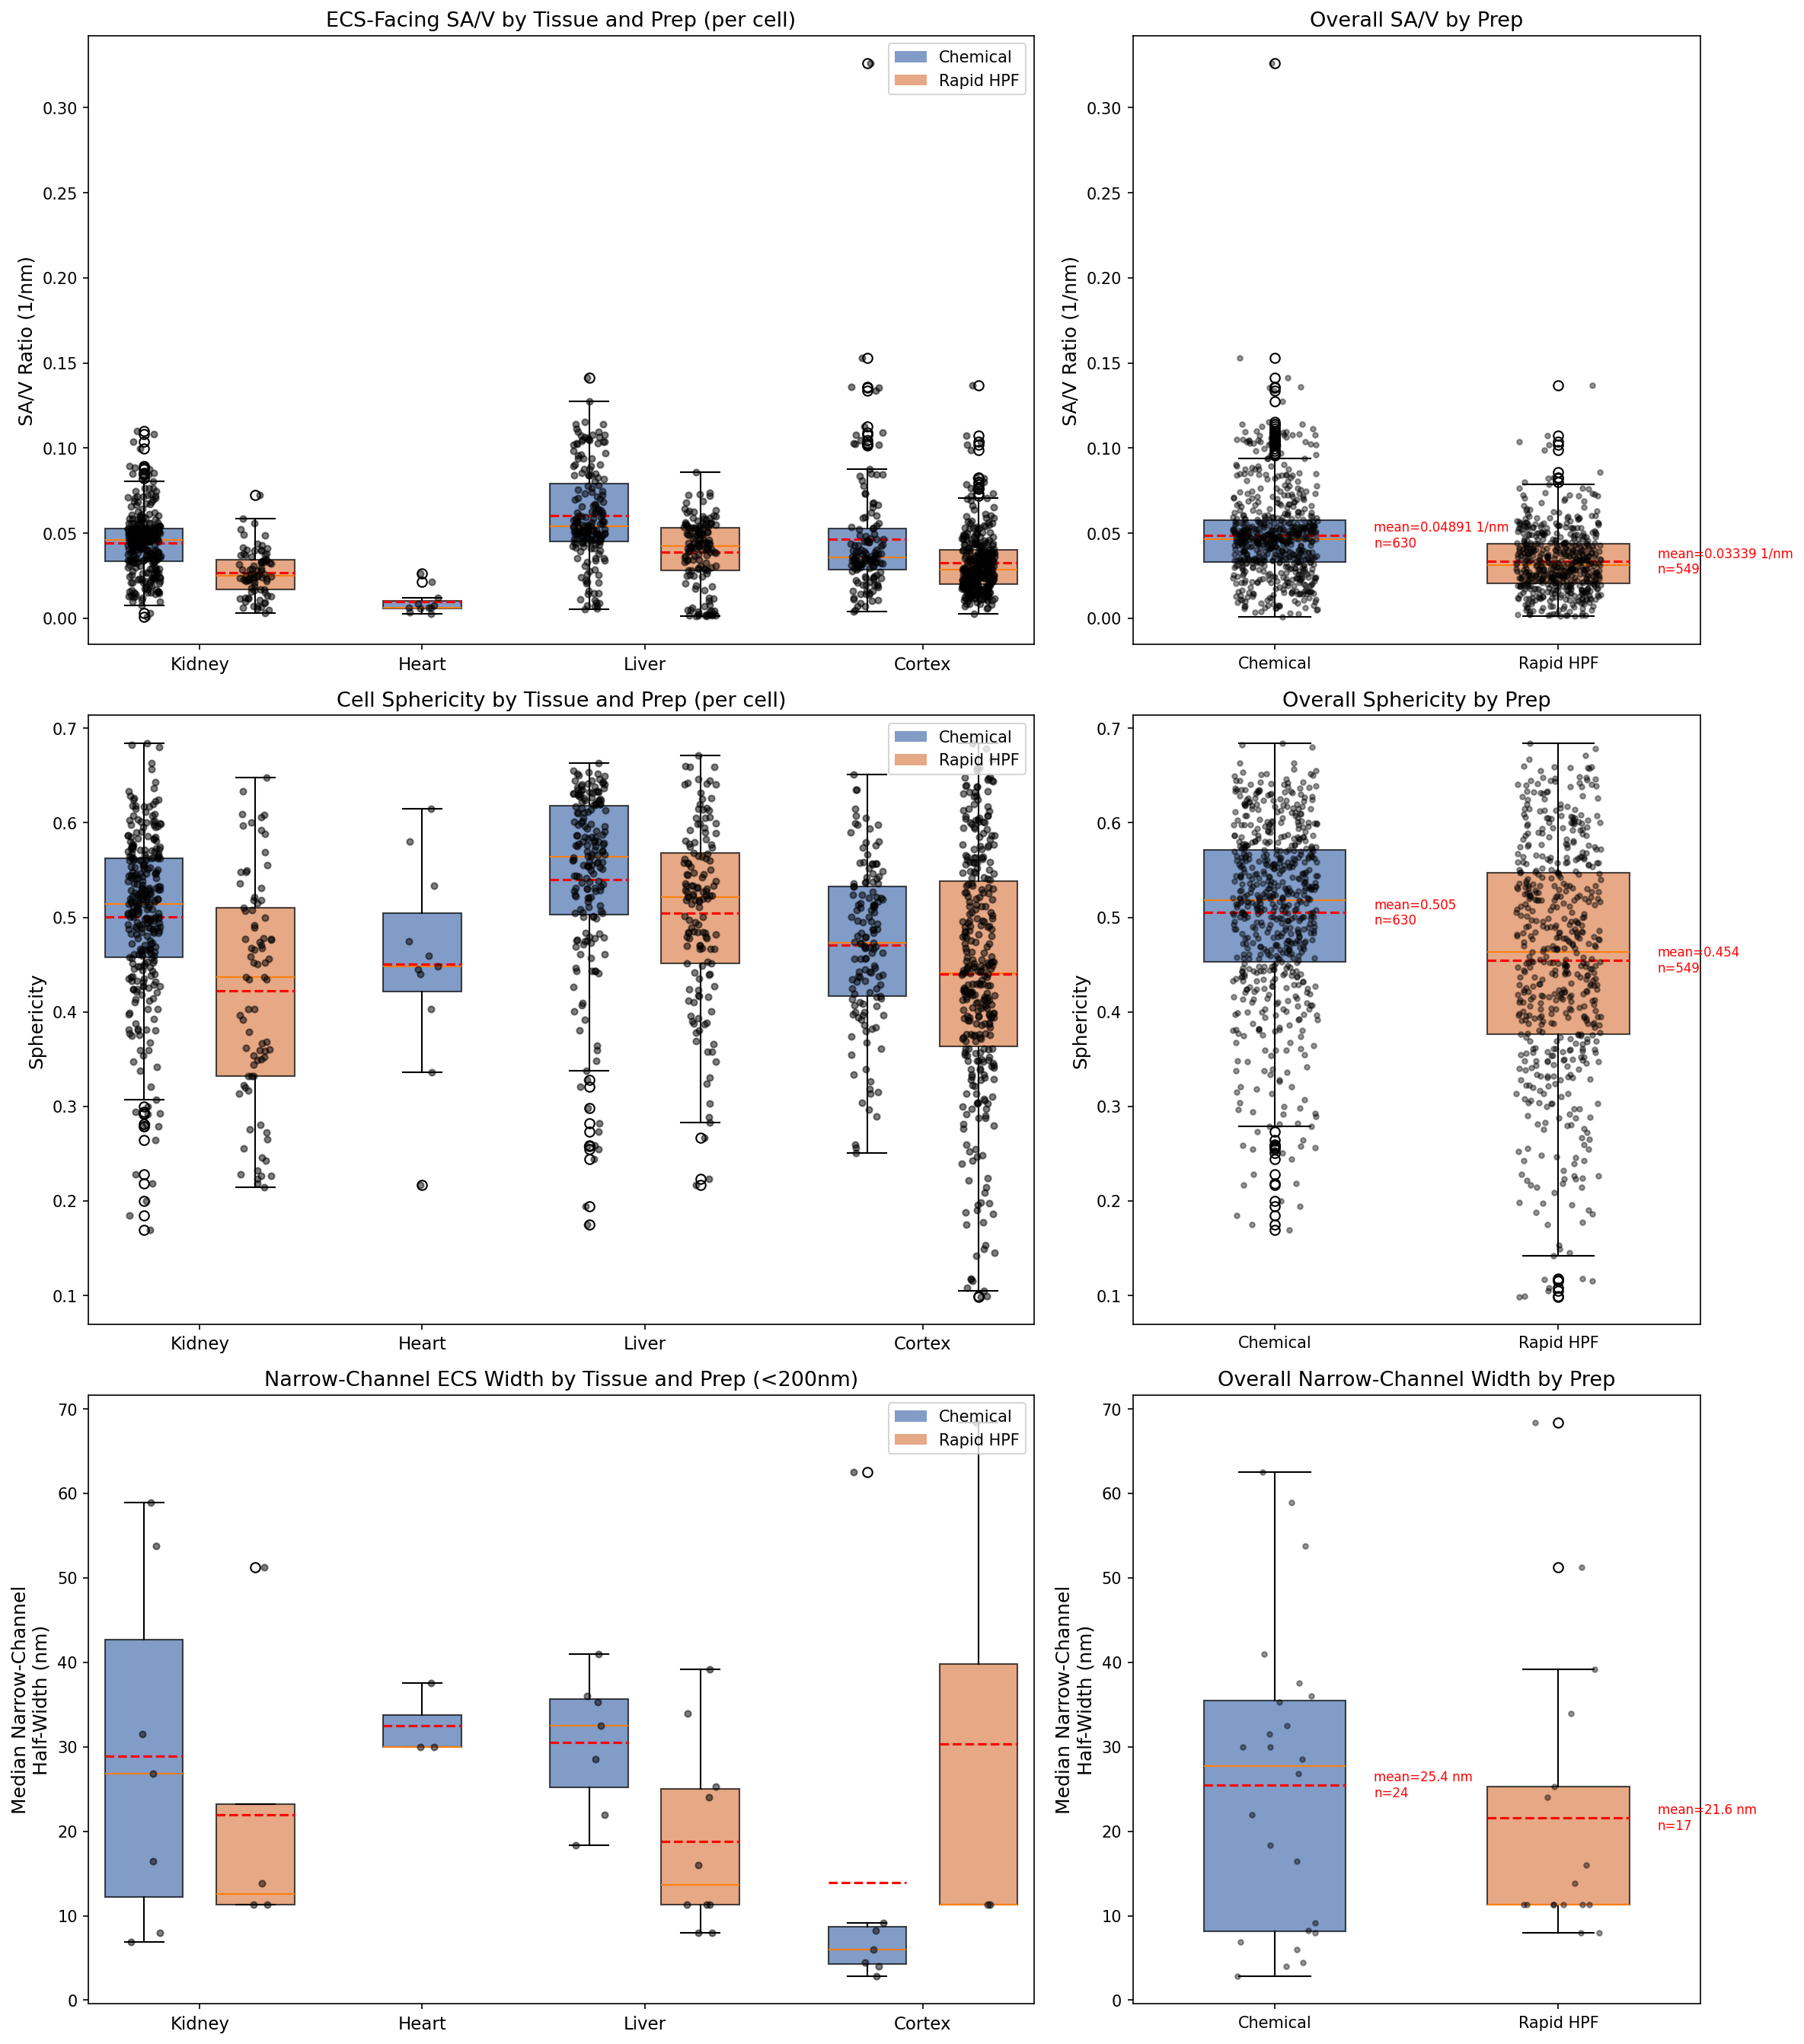
\includegraphics[width=0.95\linewidth]{Figures/cell_morphology_by_prep.png}
\caption{Per-cell morphology metrics (SA:V ratio and sphericity) by tissue and preparation type.}
\label{fig:morphology}
\end{figure*}

\begin{figure*}[t]
\centering
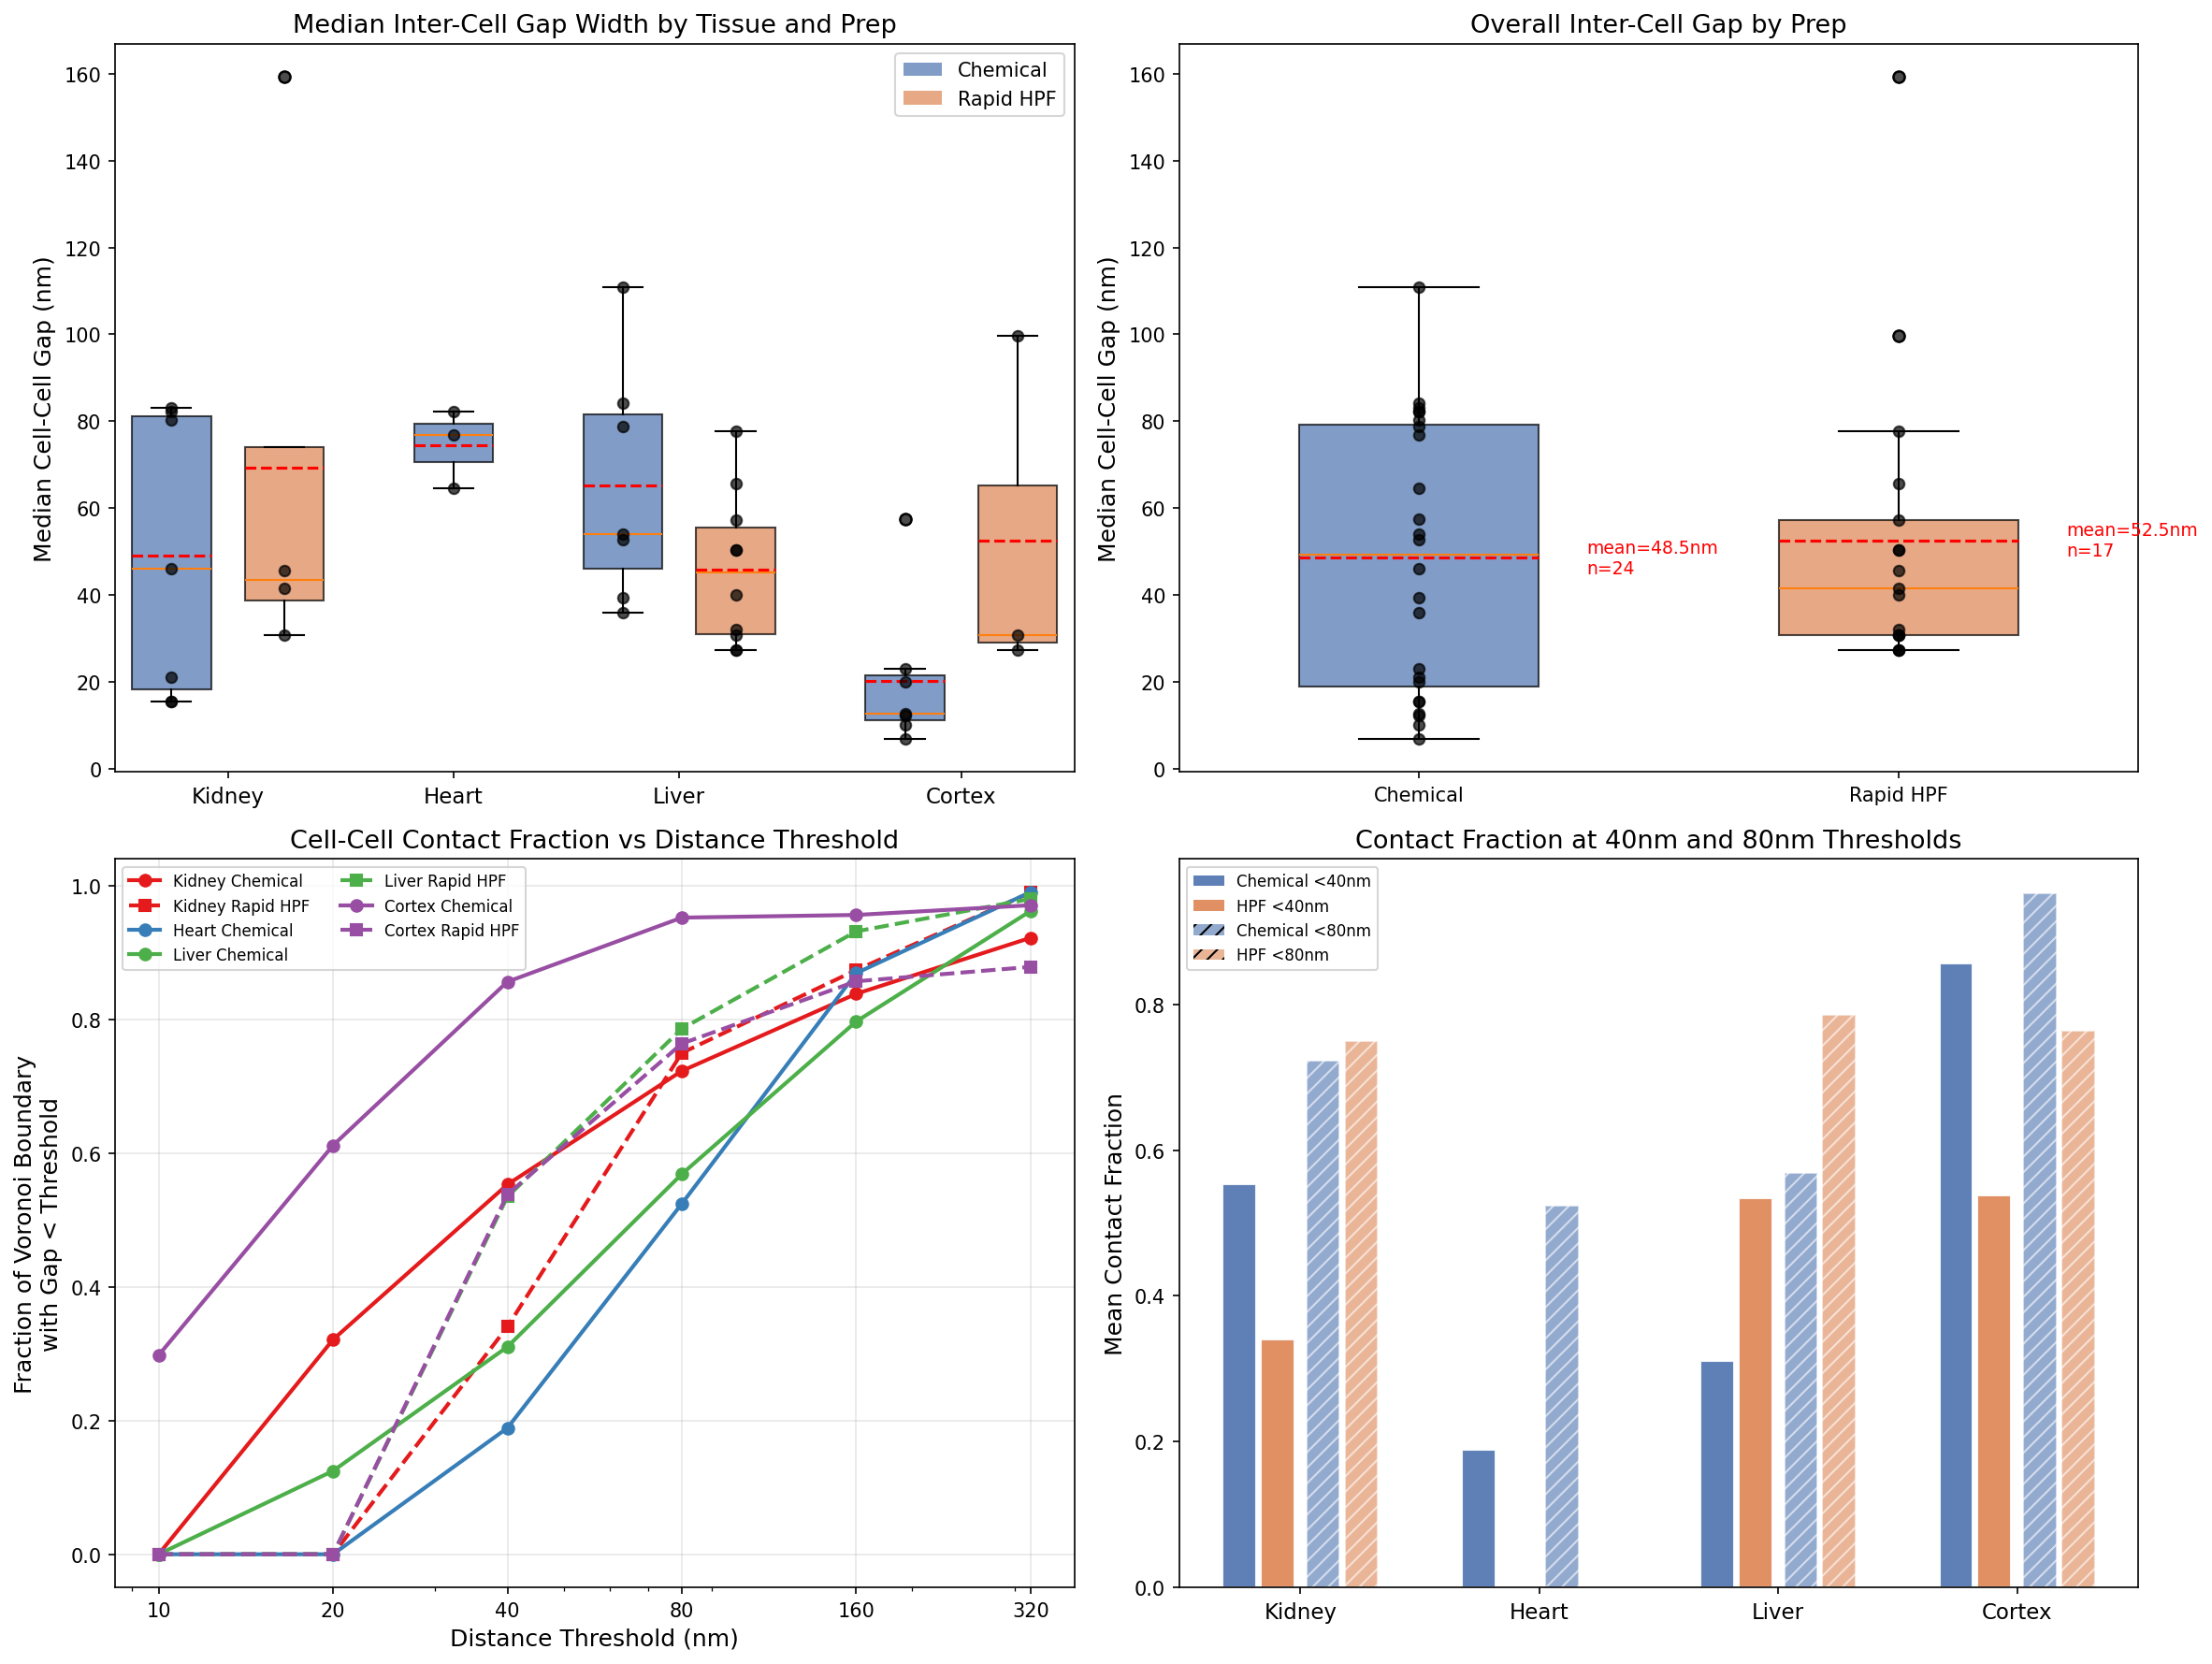
\includegraphics[width=0.95\linewidth]{Figures/cell_contacts_by_prep.png}
\caption{Inter-cell gap distance distributions and contact fractions from Voronoi tessellation of the ECS.}
\label{fig:contacts}
\end{figure*}

%% ============================================================

\begin{acknowledgements}
Data were obtained from the CellMap open-access volume EM collection (cellmap.org). % TODO: expand
\end{acknowledgements}

\section*{Bibliography}
\bibliography{references}

\end{document}
